\documentclass[10pt,a4paper]{amsart}
\usepackage[margin=19mm]{geometry}
\usepackage{amsmath,amssymb,mathtools}
\usepackage[scr=rsfs,cal=euler]{mathalfa}
\usepackage{xfrac}
\usepackage[unicode,hidelinks,bookmarks=false]{hyperref}
\newcommand{\ie}{i.e.\ }
\newcommand{\cf}{cf.\ }
\newcommand{\resp}{respectively\ }
\newcommand{\Subsection}{\subsection}
\providecommand{\nobreakdash}{\nobreak\hbox{-}}
\setlength{\emergencystretch}{2em}
\multlinegap0pt
\usepackage{tikz}
\usepackage[normalem]{ulem}
\usepackage{amssymb}
\usepackage{enumerate}
\newtheorem{theorem}{Theorem}
\newtheorem{lemma}{Lemma}
\usepackage{cleveref}
\crefname{theorem}{Theorem}{Theorems}
\crefname{lemma}{Lemma}{Lemmas}
\newcommand{\Pietro}[1]{{\color{orange}{??Pietro: #1}}} % changed to a color different from the ref blue
\newcommand{\freddy}[1]{{\color{purple}{$\spadesuit$ Freddy: #1}}}
\title{Point counts, automorphisms, and gonalities of Shimura curves}
\author{Pietro Mercuri, Oana Padurariu, Frederick Saia,, Claudio Stirpe}
\date{Source: arXiv:2507.15992v3 (CC BY 4.0)}
\begin{document}
\maketitle

\noindent\emph{Source and licence.} Point counts, automorphisms, and gonalities of Shimura curves. Version arXiv:2507.15992v3 (CC BY 4.0), distributed by arXiv under the Creative Commons Attribution 4.0 International licence, http://creativecommons.org/licenses/by/4.0/, as recorded in the arXiv licence metadata for this exact version and shown on the abstract page https://arxiv.org/abs/2507.15992v3. Full licence notice: \texttt{licenses/arxiv-2507.15992-CC-BY-4.0.txt}.\par\smallskip

\noindent\textit{Editorial scope.} Counted unit: the article's lemma CS\_geom\_hyperelliptic\_bound (source0.tex lines 730--737). The article's complete original proof of it is delivered with it (source0.tex lines 738--757, one \texttt{proof} environment of 20 lines). No mathematics is written, repaired or re-derived: the statement and the proof are the article's own lines, in the article's own notation, and no retained line is substituted or re-flowed.  Retained uncounted as the source-local context the proof needs: lines 709--719.  Nothing was omitted from any retained span, so the package carries no omission record.  No retained line contains a citation, so the wrapper carries no bibliography and no bibliography entry.  The retained lines contain the article's own diagram code, which the wrapper typesets with the standard tikz packages; no image file is delivered and the package declares no asset dependency.  Editorial formatting only, in addition: an AMS \texttt{amsart} preamble that restates the article's own declarations and macros used by the retained lines, namely the environments \texttt{theorem}, \texttt{lemma} on separate counters, together with the standard packages those lines need.  The retained environments print in this document as Theorem 1, Lemma 1 in order of appearance, whereas the article prints the same items with the numbering of its own full document.  The complete native source of the article as distributed in the arXiv e-print for this exact version is bundled unchanged as \texttt{sources/181979/source0.tex}.
\begin{theorem}[Castelnuovo--Severi]\label{theorem: CS}
Let $F$ be a perfect field and let $X$, $Y$, and $Z$ be curves over $F$. Let
\[
\pi_Y\colon X \to Y\qquad\text{and} \qquad \pi_Z\colon X \to Z
\]
be non-constant morphisms defined over $F$. Then either
\[
g(X) \leq \textnormal{deg}(\pi_Y)\cdot g(Y) + \textnormal{deg}(\pi_Z)\cdot g(Z) + (\textnormal{deg}(\pi_Y)-1)(\textnormal{deg}(\pi_Z)-1),
\]
or there exists a curve $X'$ over $F$ and a morphism $X \to X'$ over $F$ of degree greater than $1$ through which both $\pi_Y$ and $\pi_Z$ factor. 
\end{theorem}

\begin{lemma}\label{lemma: CS_geom_hyperelliptic_bound}
Let $X$ be a curve of genus~$g$ over a perfect field~$F$ possessing an involution~$\sigma$, %\Pietro{over $F$?}
and suppose that the genus $g_\sigma$ of the quotient $X/\langle \sigma \rangle$ satisfies $g_\sigma > 0$. If
\[
g > 2g_\sigma + 1,
\]
then $X$ is not geometrically hyperelliptic. 
\end{lemma}

\begin{proof}
Let $q\colon X \to X/\langle \sigma \rangle$ denote the natural quotient map. Suppose to the contrary that there is a degree~$2$ map $f\colon X \to C$ to a conic~$C$. Because of the assumed strict inequality, \cref{theorem: CS} tells us that we must have a commutative diagram of the following shape over~$F$
\[
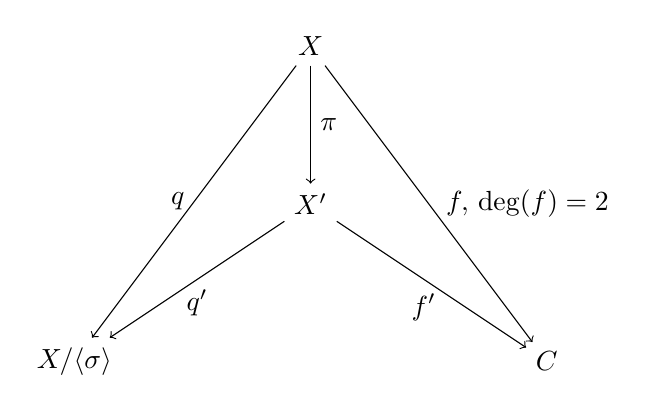
\begin{tikzpicture}[node distance=2.2cm]
\node (X) at (0,2) {$X$};
\node (Xp) at (0,0) {$X'$};
\node (Q) at (-3,-2) {$X/\langle \sigma \rangle$};
\node (C) at (3,-2) {$C$};

\draw[->] (X) -- node[right] {$\pi$} (Xp);
\draw[->] (X) -- node[left] {$q$} (Q);
\draw[->] (X) -- node[right] {$\;f,\, \deg(f) = 2$} (C);
\draw[->] (Xp) -- node[below] {$q'$} (Q);
\draw[->] (Xp) -- node[below] {$f'\;\;$} (C);
\end{tikzpicture}
\]
with $\deg(\pi) > 1$. Hence $\deg(\pi) = 2$ and $q'$ and $f'$ are both isomorphisms, which implies that 
\[ g\left(X/\langle \sigma \rangle\right) = g(C) = 0 \]
and contradicts our hypothesis. %\freddy{I've tried to clarify this argument (including your diagram -- thanks!). Feel free to further comment or adjust things!}
\end{proof}

\end{document}
